\chapter{A}
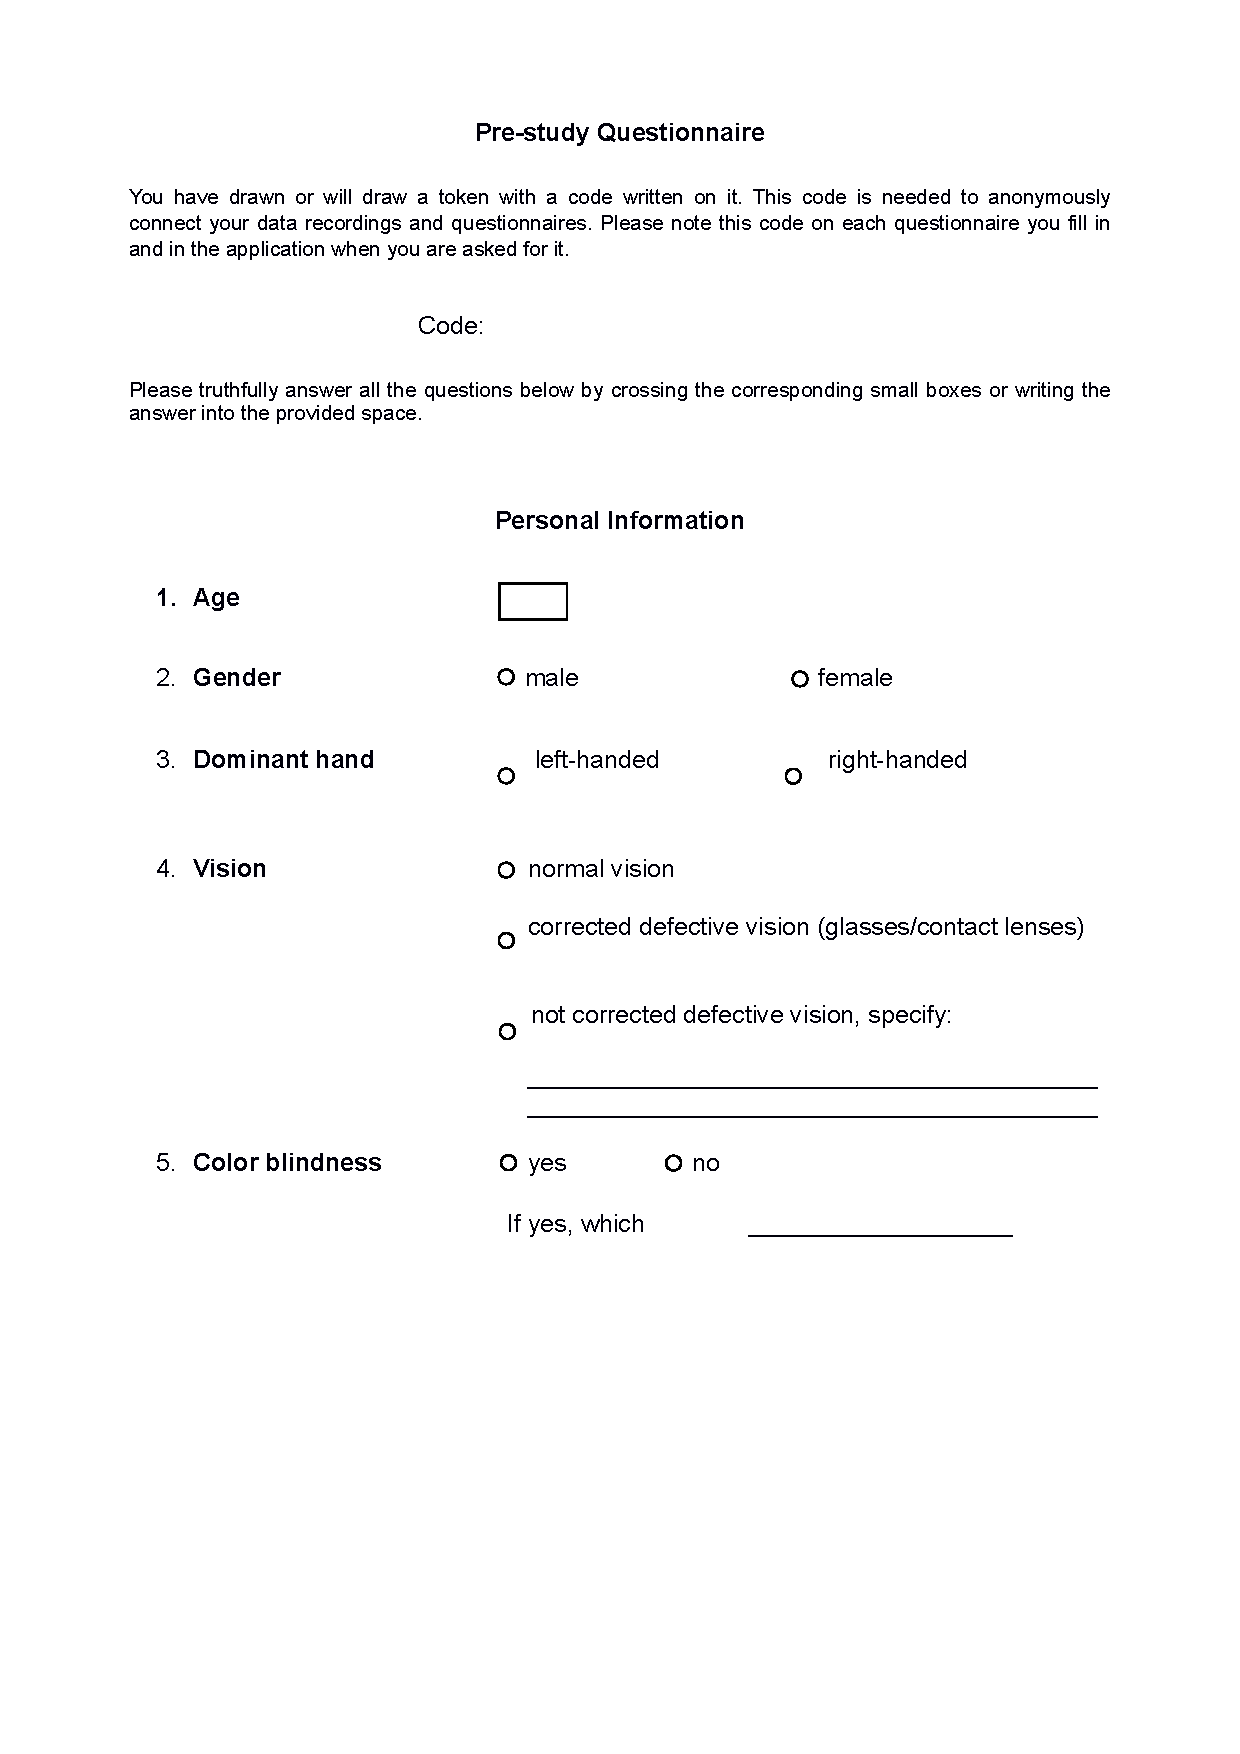
\includepdf[pages=-]{appendix/PreStudy.pdf}
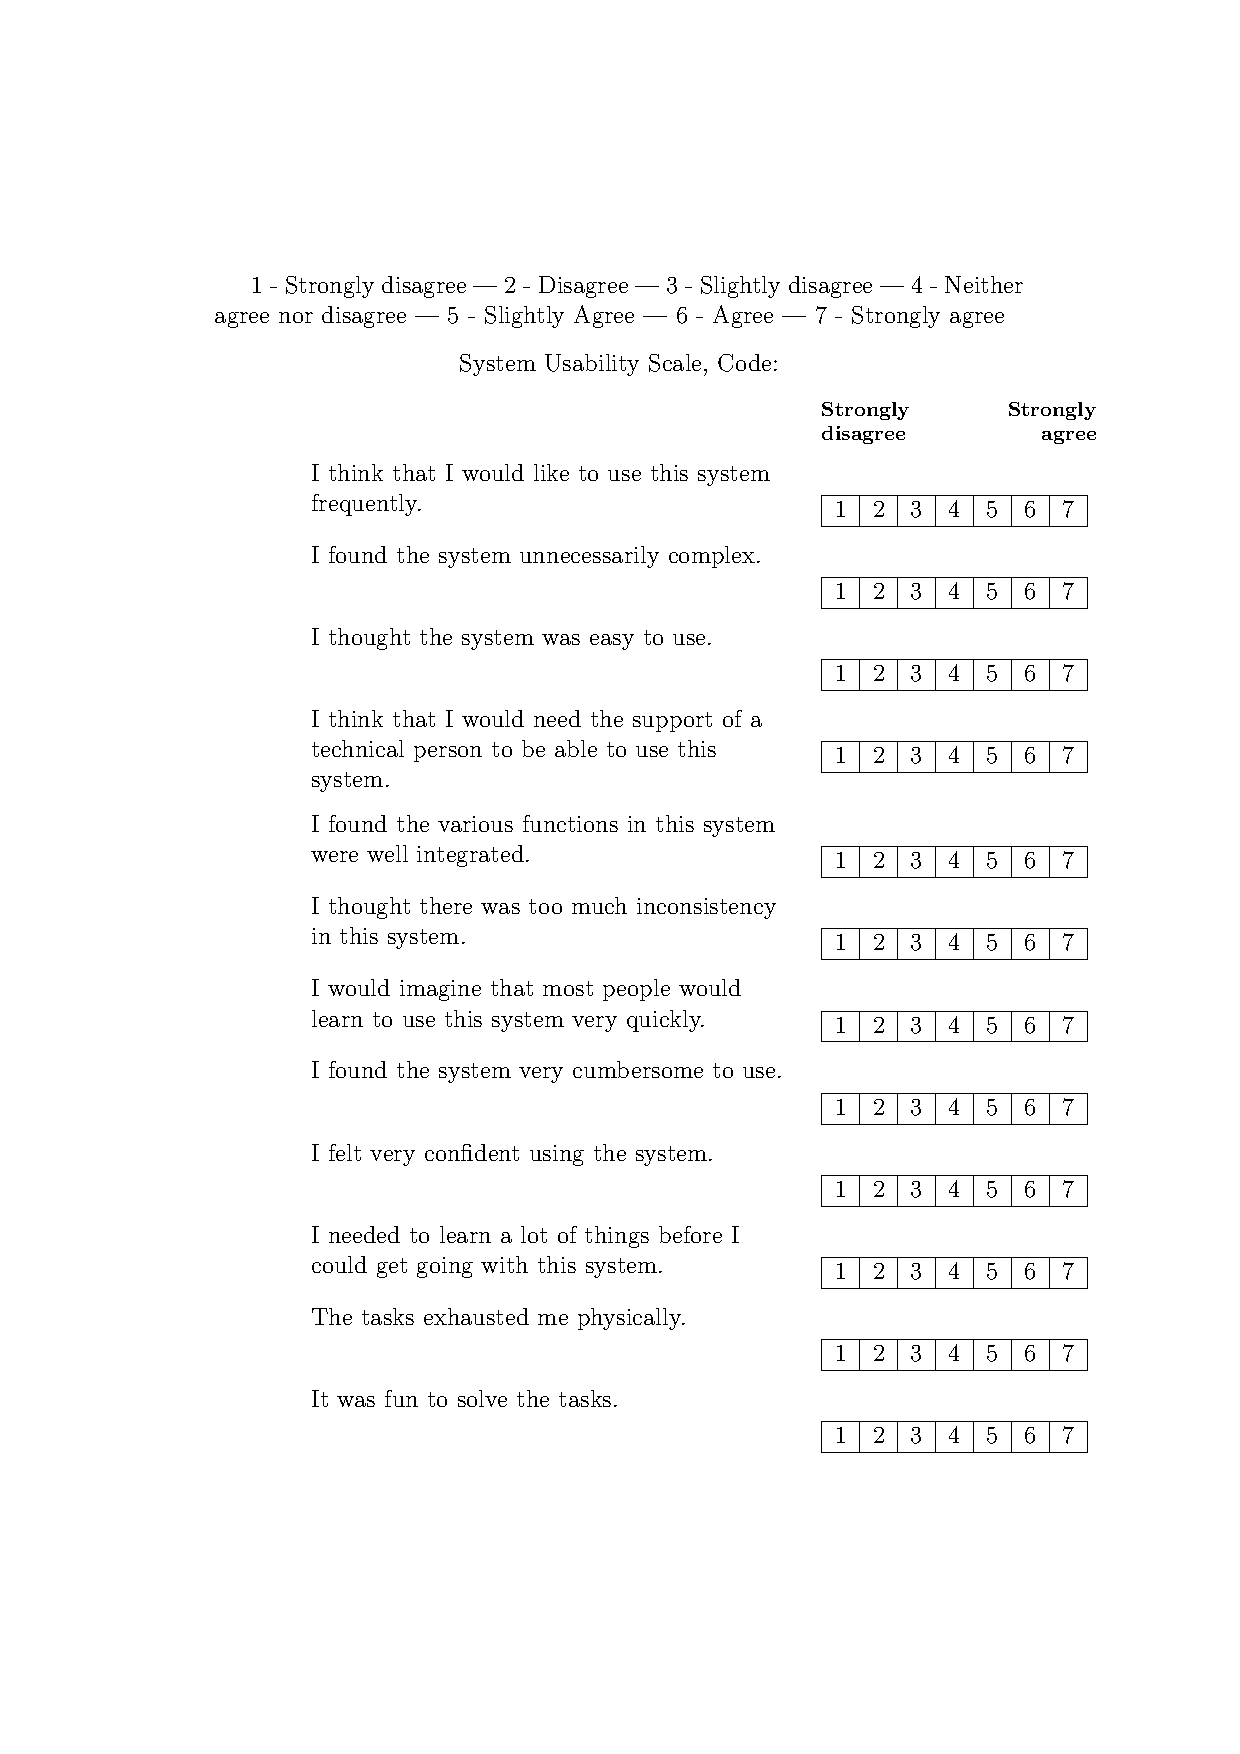
\includepdf[pages=-]{appendix/questionnaire.pdf}

\chapter{B}
\begin{table}[t]
    \centering
    \begin{tabular}{llllllllll}
    \textbf{Participant} & \textbf{AGE} & \textbf{GENDER} & \textbf{HANDED} & \textbf{VISION} & \textbf{COLOR\_BLINDNESS} & \textbf{Q6} & \textbf{Q7} & \textbf{Q8} & \textbf{Q9} \\
    1             & 32           & M               & RIGHT           & NORMAL          & FALSE                     & B           & A           & C           & C           \\
    2             & 34           & M               & LEFT            & NORMAL          & FALSE                     & B           & B           & B           & B           \\
    3             & 28           & M               & RIGHT           & NORMAL          & FALSE                     & B           & B           & B           & B           \\
    4             & 32           & M               & RIGHT           & CORRECTED       & FALSE                     & B           & C           & C           & C           \\
    5             & 34           & M               & RIGHT           & CORRECTED       & FALSE                     & C           & B           & C           & C          
    \end{tabular}
\end{table}